%%% template.tex
%%%
%%% This LaTeX source document can be used as the basis for your technical
%%% paper or abstract.

%%% The parameter to the ``documentclass'' command is very important.
%%% - use ``review'' for content submitted for review.
%%% - use ``preprint'' for accepted content you are making available.
%%% - use ``tog'' for technical papers accepted to the TOG journal and
%%%   for presentation at the SIGGRAPH or SIGGRAPH Asia conference.
%%% - use ``conference'' for final content accepted to a sponsored event
%%%   (hint: If you don't know, you should use ``conference.'')

\documentclass[tog]{acmsiggraph}

%%% Make the ``BibTeX'' word pretty...

\def\BibTeX{{\rm B\kern-.05em{\sc i\kern-.025em b}\kern-.08em
    T\kern-.1667em\lower.7ex\hbox{E}\kern-.125emX}}

%%% Used by the ``review'' variation; the online ID will be printed on 
%%% every page of the content.

\TOGonlineid{45678}

%%% Used by the ``preprint'' variation.

\TOGvolume{0}
\TOGnumber{0}

\title{Rendering Project}

\author{Marta Feriani\\MSc Computer Animation and Visual Effects}
\pdfauthor{Marta Feriani}

\keywords{RenderManProServer20, shading, modelling}

\begin{document}

%%% This is the ``teaser'' command, which puts an figure, centered, below 
%%% the title and author information, and above the body of the content.

 \teaser{
   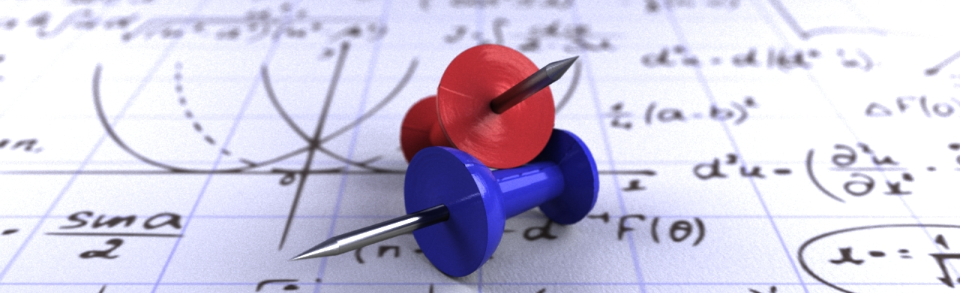
\includegraphics[width=6.5in]{images/teaser}
   \caption{Final image}
 }

\maketitle

\begin{abstract}

In this paper we describe the process of creating a photo realistic thumb tack using RenderMan 20. The paper will first present graphic references for the object and will then proceed with a detailed analysis of the production process.
Aspect such as modelling, shading and light models will be considered.

\end{abstract}

\keywordlist

%% Required for all content. 

\copyrightspace



\section{Modelling a thumb tack}

The thumb tack provided to be a suitable object for this project. Its shape resulted to be simple enough to be reproduced using RenderMan's built-in primitives yet interesting for the variety of different primitives needed.

The metal part was reconstructed using basic shapes such as a cone and a cylinder.
The plastic part presented more interesting features such as the curved part connecting with the metal stick or the main plastic body. Looking closely at the real model plastic body, primitives such cylinders and cones were found not to be accurate enough to be used to faithfully reproduce the original silhouette.
The final model consisted eventually of a flat hyperboloid to cover the base of the plastic body. An horizontal section of a sphere represented the curved part. On top of it, three different sized hyperboloids were used to achieved the main look for the thumb tack. The top part of the model was then closed with a disk.

\begin{figure}[h]
  \centering
  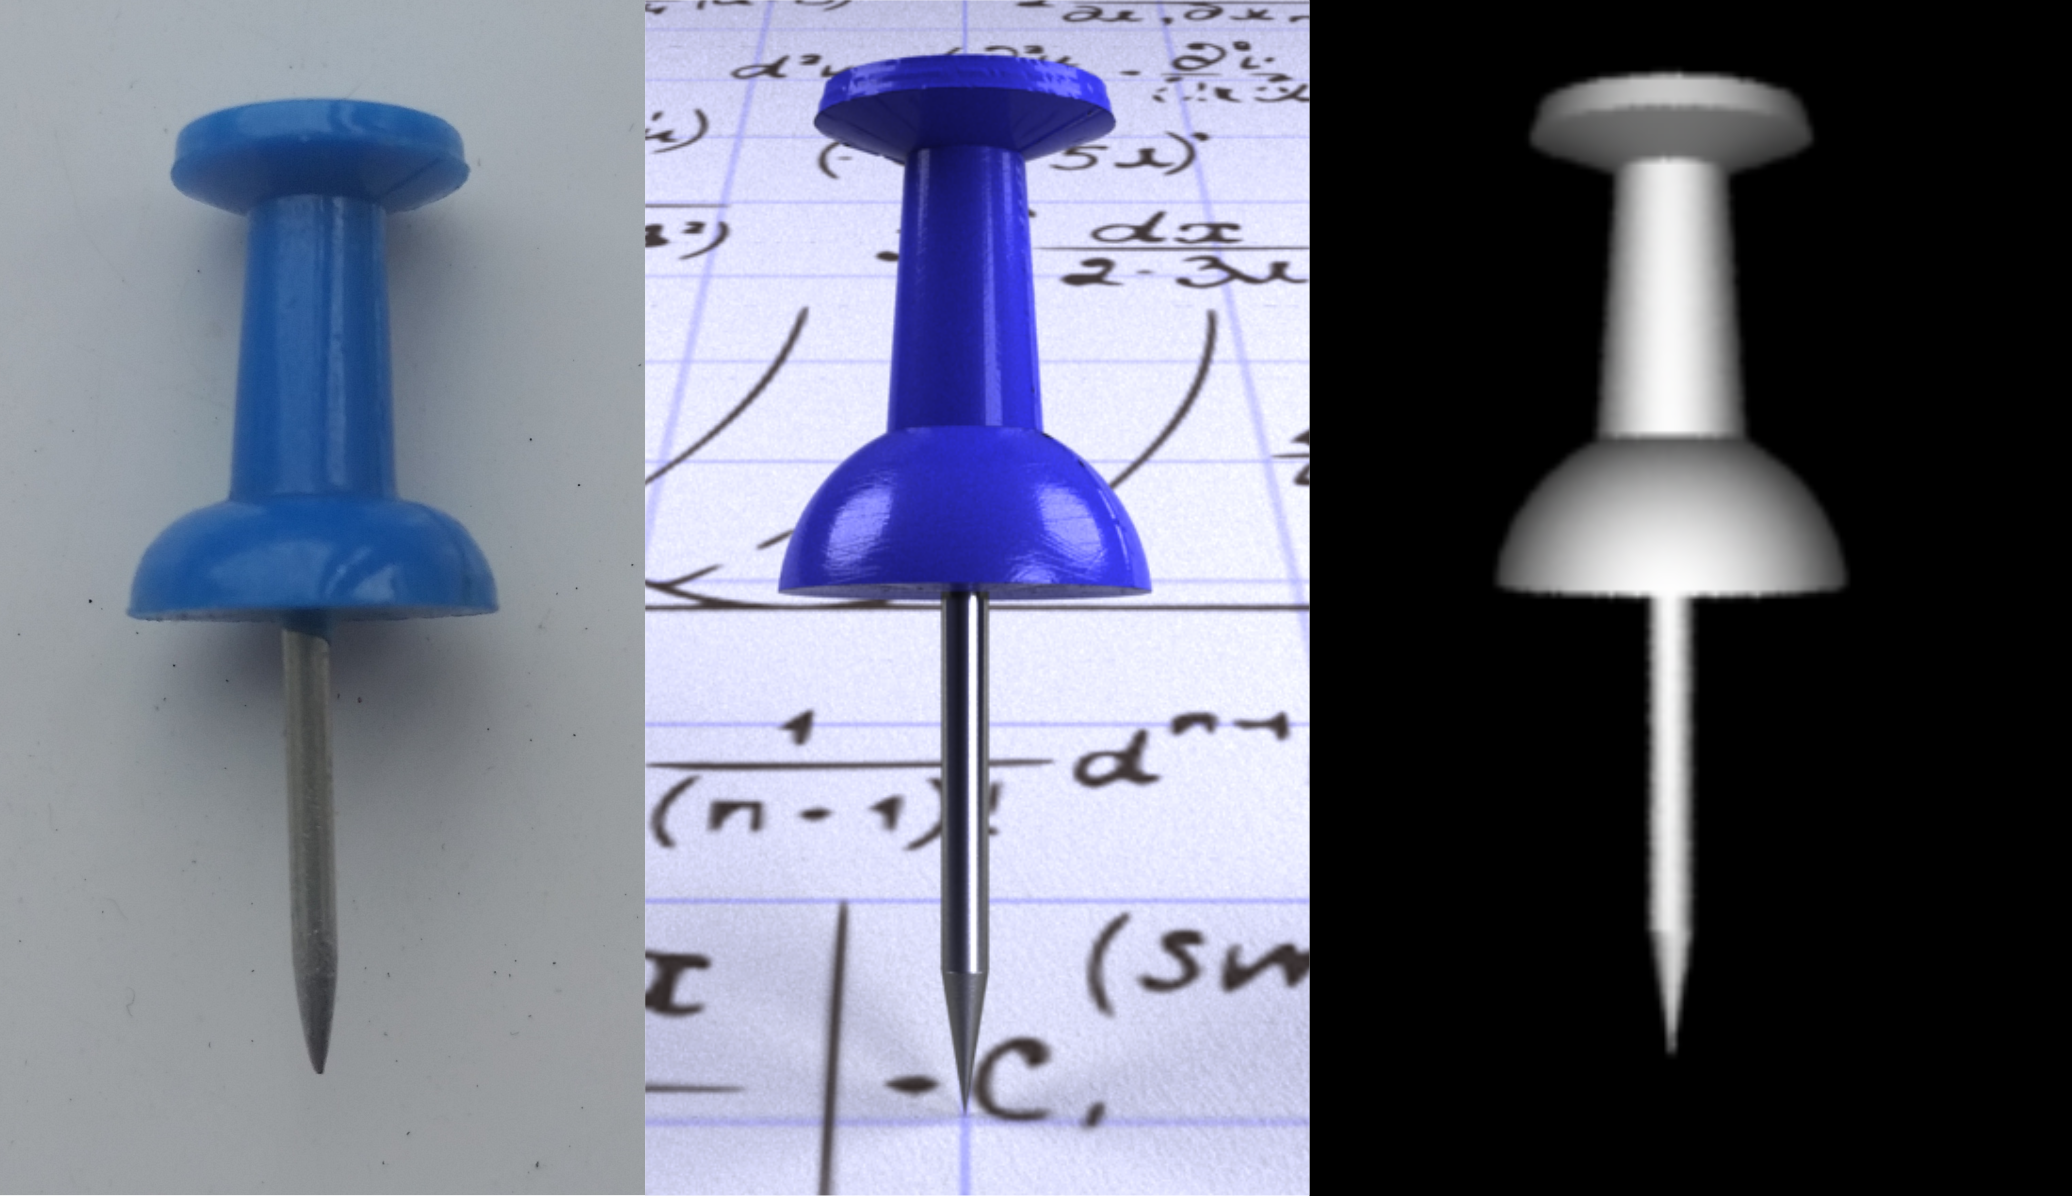
\includegraphics[width=6.3cm]{images/modelling.png}
  \caption{Comparison: real model and computer generated geometry.}
  \label{fig:modelling}
\end{figure}

\vspace{1.0cm}
The modelling process started by measuring each section of the real model. When recreating it, I tried to replicate the same values for width and length for each piece of geometry. Even though I first thought this to be the most precise approach, the result was not close enough to the real model, probably because the measurements themselves lacked the required level of precision.
Those measurements have hence been tweaked to achieve a better outcome.

\begin{figure}[h!]
  \centering
  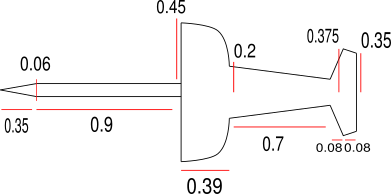
\includegraphics[width=3.0in]{images/measurements.png}
  \caption{Some measurements on the models}
  \label{fig:measurements}
\end{figure}

\newpage
\section{Materials}

In the scene we can identify three different materials such as plastic, metal and paper.

\subsection{Plastic}
When analyzing the real model in details, the surface appeared to be extremely smooth and shiny despite small scratches and imperfections spread across the surface. To correctly reproduce the base material, the \texttt{bxdf} RenderMan model was used, setting \texttt{clearcoat} and \texttt{specular} to \texttt{1} while the \texttt{roughness} value to \texttt{0}.

\subsection{Metal}
The metal stick presented a varying roughness along the surface, being more noticeable on the pointy tip. The material was recreated using the \texttt{bxdf} material and setting the \texttt{metallic} property value to \texttt{1} for both the stick and pointy end, while the roughness was varied along the surface using a shader to achieve a look closer to the original model.

\subsection{Paper\label{paper}}
The paper I wanted to include in my scene was a type of thick, rough paper normally used for watercolours paintings. To try and recreate a material with the same look I decided to rely on a shader for the small bumps across the surface while achieving the material properties using again the \texttt{bxdf} material with \texttt{roughness} set to \texttt{0.5} and specular to \texttt{0.1}.

\section{Pattern and Displacements}

The project uses primarily displacements shaders. Each displacement pattern is described in a different surface shader. The output of the pattern produced is then fed in a displacement shader that translates the pattern into an evaluation of mesh points position and re-evaluates the normal on the surface. While each pattern is produced by a different shader, the conversion is handled by a unique displacement shader.

\subsection{Wave.osl}

The purpose of this shader was to successfully reproduce the vertical junction line that joins the two half of the plastic part together.
The junction presents a straight direction with jagged edges and wear marks. Therefore the shader consists of:

\begin{itemize}
  \item $sin$ function that takes as argument the $u$ coordinate and a repetition value. This creates periodical vertical creases on the surface.
  \item The $sin$ function is the fed in the abs() function to double the frequency of the creases by mirroring the negative areas of the sin function to the positive.
  \item the $smoothstep$ function is then applied to narrow the creases and make their width constant along the curve.
\end{itemize}

The previous steps managed to achieve the creases, even though they looked too sharp and unreal. To overcome the problem two layers of noise at different frequencies have been added on top.

The shader allows the user to specify the number of creases and the displacement amount on the surface.

\begin{figure}[ht]
  \centering
  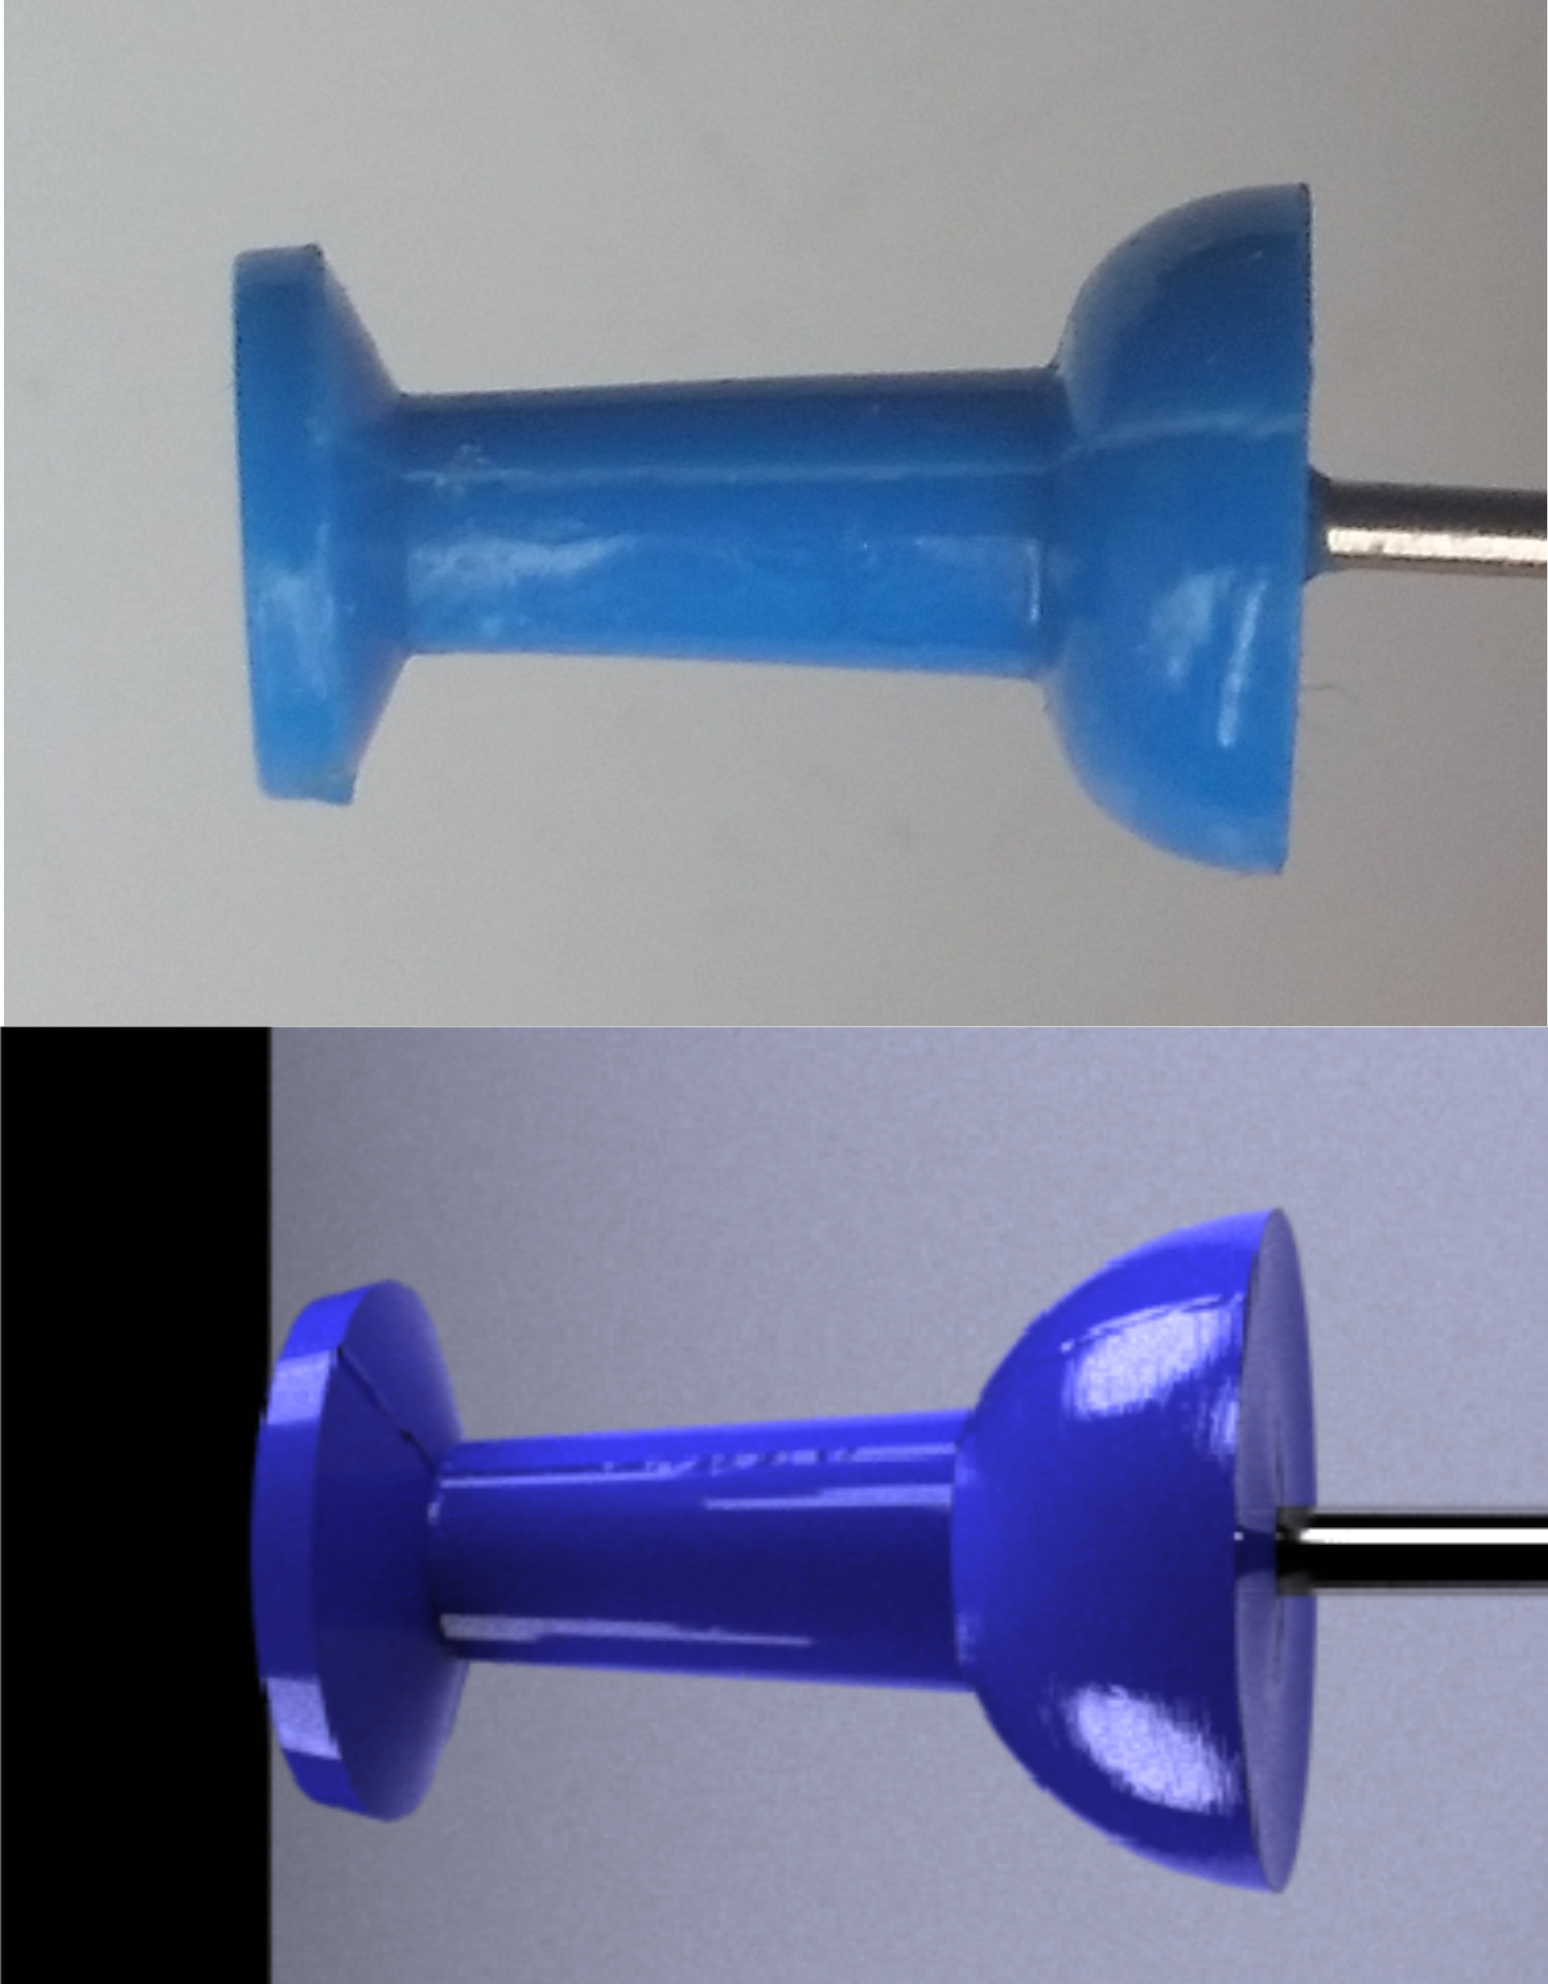
\includegraphics[width=3.0in]{images/wave.png}
  \caption{Longitudinal creases achieved with wave shader}
  \label{fig:wave}
\end{figure}

\subsection{Topdisk.osl}

The shader aims to create a small depressed area on the top of the thumb tack. The model top disk appears to be flat around the edges while concave in the central area. The result is achieved using a smoothstep function starting from half of the radius distance from the center and the center itself.

\begin{figure}[h!]
  \centering
  \includegraphics[width=3.0in]{images/topdisk.png}
  \caption{Concave area around the center}
  \label{fig:topdisk}
\end{figure}

\newpage
\subsection{Disk.osl}

The disk was created for the thumb tack lower plastic part. In the beginning it was applied on a disk geometry but later during the project I remodeled it using a flat hyperboloid instead. The change was due to the difficulties that arose when shading the junction between the plastic and metal elements. The hyperboloid shape allowed me to have a hole in the middle with a radius that matched the metal pin one. The shader creates a first layer that deforms the surface according to the cosine function. Adjustments in the phase have been made to keep the position of the external edges unchanged. A displacement of the edge points would have lead to breaking the model. As a second layer, noise in the \texttt{v} coordinates achieves the creases in the radial direction.

\begin{figure}[ht]
  \centering
  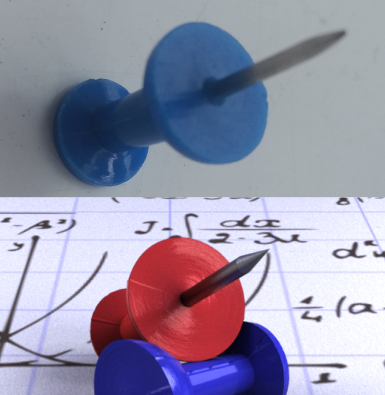
\includegraphics[height=2.9in]{images/disk.png}
  \caption{Longitudinal creases achieved with wave shader}
  \label{fig:disk}
\end{figure}

\subsection{paper.osl}

To achieve the rough paper look described in~\ref{paper} I used a simple noise in one direction. The first attempt using Perlin noise resulted in artifacts that affected the final picture. The high frequency of the noise probably being greater than the Nyquist limit may have been the cause for the aliasing distortions. The issue was solved by using a simplex noise at lower frequency instead.

\begin{figure}[ht]
  \centering
  
\includegraphics[width=3.0in]{images/paper.png}
  \caption{Left: real paper. Right: paper generated with a displacement shader}
  \label{fig:paper}
\end{figure}

\vspace{1.0cm}
\subsection{metal.osl}

The metal shader changes the roughness value along the metal stick allowing a smooth transition between the rough pin point to the smoother end. The transition is achieved using a mix function.

To make the final look more realistic, I used a texture as bump map to add scratches along the surface, using different scale values to fit the geometry current geometry.

\section{Scene composition}

As final shot composition, I arranged the scene as a macro image. I wanted it to be uniformly lit as it was staged in a modern office. The lighting in the scene consists therefore of an area light that provides the main light source and three different glowing sphere positioned at the sides of the object. To give the illusion of the object being placed in an office, I first tried to use a \texttt{PxrStdEnvMapLight} but the result was not satisfying. A shader that transferred the environment map to the reflection on the surfaces of the object managed to create the proper atmosphere. Other attempts to tune the atmosphere were done by changing the temperature of the light, even though they have not been used for the final pictures.

The staging at this level of production was still missing depth. The object was made to stand out using the depth of field option. The tuning the three variables was carried on a trial and error basis. The final values was 5.6 for the \texttt{fstop}, 0.9 as \texttt{focal length} and \texttt{focal distance} of 6.8.

\begin{figure}[ht]
  \centering
  \includegraphics[width=3.0in]{images/blur}
  \caption{Depth of field stages of production}
  \label{fig:blur}
\end{figure}

\end{document}
